\documentclass[twoside]{book}

% Packages required by doxygen
\usepackage{fixltx2e}
\usepackage{calc}
\usepackage{doxygen}
\usepackage[export]{adjustbox} % also loads graphicx
\usepackage{graphicx}
\usepackage[utf8]{inputenc}
\usepackage{makeidx}
\usepackage{multicol}
\usepackage{multirow}
\PassOptionsToPackage{warn}{textcomp}
\usepackage{textcomp}
\usepackage[nointegrals]{wasysym}
\usepackage[table]{xcolor}

% Font selection
\usepackage[T1]{fontenc}
\usepackage[scaled=.90]{helvet}
\usepackage{courier}
\usepackage{amssymb}
\usepackage{sectsty}
\renewcommand{\familydefault}{\sfdefault}
\allsectionsfont{%
  \fontseries{bc}\selectfont%
  \color{darkgray}%
}
\renewcommand{\DoxyLabelFont}{%
  \fontseries{bc}\selectfont%
  \color{darkgray}%
}
\newcommand{\+}{\discretionary{\mbox{\scriptsize$\hookleftarrow$}}{}{}}

% Page & text layout
\usepackage{geometry}
\geometry{%
  a4paper,%
  top=2.5cm,%
  bottom=2.5cm,%
  left=2.5cm,%
  right=2.5cm%
}
\tolerance=750
\hfuzz=15pt
\hbadness=750
\setlength{\emergencystretch}{15pt}
\setlength{\parindent}{0cm}
\setlength{\parskip}{3ex plus 2ex minus 2ex}
\makeatletter
\renewcommand{\paragraph}{%
  \@startsection{paragraph}{4}{0ex}{-1.0ex}{1.0ex}{%
    \normalfont\normalsize\bfseries\SS@parafont%
  }%
}
\renewcommand{\subparagraph}{%
  \@startsection{subparagraph}{5}{0ex}{-1.0ex}{1.0ex}{%
    \normalfont\normalsize\bfseries\SS@subparafont%
  }%
}
\makeatother

% Headers & footers
\usepackage{fancyhdr}
\pagestyle{fancyplain}
\fancyhead[LE]{\fancyplain{}{\bfseries\thepage}}
\fancyhead[CE]{\fancyplain{}{}}
\fancyhead[RE]{\fancyplain{}{\bfseries\leftmark}}
\fancyhead[LO]{\fancyplain{}{\bfseries\rightmark}}
\fancyhead[CO]{\fancyplain{}{}}
\fancyhead[RO]{\fancyplain{}{\bfseries\thepage}}
\fancyfoot[LE]{\fancyplain{}{}}
\fancyfoot[CE]{\fancyplain{}{}}
\fancyfoot[RE]{\fancyplain{}{\bfseries\scriptsize Generated by Doxygen }}
\fancyfoot[LO]{\fancyplain{}{\bfseries\scriptsize Generated by Doxygen }}
\fancyfoot[CO]{\fancyplain{}{}}
\fancyfoot[RO]{\fancyplain{}{}}
\renewcommand{\footrulewidth}{0.4pt}
\renewcommand{\chaptermark}[1]{%
  \markboth{#1}{}%
}
\renewcommand{\sectionmark}[1]{%
  \markright{\thesection\ #1}%
}

% Indices & bibliography
\usepackage{natbib}
\usepackage[titles]{tocloft}
\setcounter{tocdepth}{3}
\setcounter{secnumdepth}{5}
\makeindex

% Hyperlinks (required, but should be loaded last)
\usepackage{ifpdf}
\ifpdf
  \usepackage[pdftex,pagebackref=true]{hyperref}
\else
  \usepackage[ps2pdf,pagebackref=true]{hyperref}
\fi
\hypersetup{%
  colorlinks=true,%
  linkcolor=blue,%
  citecolor=blue,%
  unicode%
}

% Custom commands
\newcommand{\clearemptydoublepage}{%
  \newpage{\pagestyle{empty}\cleardoublepage}%
}

\usepackage{caption}
\captionsetup{labelsep=space,justification=centering,font={bf},singlelinecheck=off,skip=4pt,position=top}

%===== C O N T E N T S =====

\begin{document}

% Titlepage & ToC
\hypersetup{pageanchor=false,
             bookmarksnumbered=true,
             pdfencoding=unicode
            }
\pagenumbering{alph}
\begin{titlepage}
\vspace*{7cm}
\begin{center}%
{\Large M\+PE }\\
\vspace*{1cm}
{\large Generated by Doxygen 1.8.13}\\
\end{center}
\end{titlepage}
\clearemptydoublepage
\pagenumbering{roman}
\tableofcontents
\clearemptydoublepage
\pagenumbering{arabic}
\hypersetup{pageanchor=true}

%--- Begin generated contents ---
\chapter{M\+PE}
\label{md__m_p_e__r_e_a_d_m_e}
\Hypertarget{md__m_p_e__r_e_a_d_m_e}
Message Passing Engine 
\chapter{Class Index}
\section{Class List}
Here are the classes, structs, unions and interfaces with brief descriptions\+:\begin{DoxyCompactList}
\item\contentsline{section}{\hyperlink{struct_tag}{Tag} }{\pageref{struct_tag}}{}
\item\contentsline{section}{\hyperlink{class_m_p_e_1_1_thread}{M\+P\+E\+::\+Thread} \\*The thread base class }{\pageref{class_m_p_e_1_1_thread}}{}
\item\contentsline{section}{\hyperlink{class_m_p_e_1_1_thread_message_controller}{M\+P\+E\+::\+Thread\+Message\+Controller} \\*The \hyperlink{class_m_p_e_1_1_thread_message_controller}{Thread\+Message\+Controller} initiates threads and handles the communication between them }{\pageref{class_m_p_e_1_1_thread_message_controller}}{}
\end{DoxyCompactList}

\chapter{Class Documentation}
\hypertarget{struct_tag}{}\section{Tag Struct Reference}
\label{struct_tag}\index{Tag@{Tag}}


{\ttfamily \#include $<$M\+P\+E\+\_\+\+Tag.\+h$>$}

\subsection*{Static Public Attributes}
\begin{DoxyCompactItemize}
\item 
\mbox{\Hypertarget{struct_tag_a912b98789132f59ca299c8a98d649a16}\label{struct_tag_a912b98789132f59ca299c8a98d649a16}} 
static const uint32\+\_\+t {\bfseries Any} = 0
\item 
\mbox{\Hypertarget{struct_tag_a92d980ab77af22009b018f020cf39d23}\label{struct_tag_a92d980ab77af22009b018f020cf39d23}} 
static const uint32\+\_\+t {\bfseries Shutdown} = 1
\end{DoxyCompactItemize}


\subsection{Detailed Description}
The basic tags used during message passing. 

The documentation for this struct was generated from the following file\+:\begin{DoxyCompactItemize}
\item 
M\+P\+E\+\_\+\+Tag.\+h\end{DoxyCompactItemize}

\hypertarget{class_m_p_e_1_1_thread}{}\section{M\+PE\+:\+:Thread Class Reference}
\label{class_m_p_e_1_1_thread}\index{M\+P\+E\+::\+Thread@{M\+P\+E\+::\+Thread}}


The thread base class.  




{\ttfamily \#include $<$Thread.\+h$>$}

Inheritance diagram for M\+PE\+:\+:Thread\+:\begin{figure}[H]
\begin{center}
\leavevmode
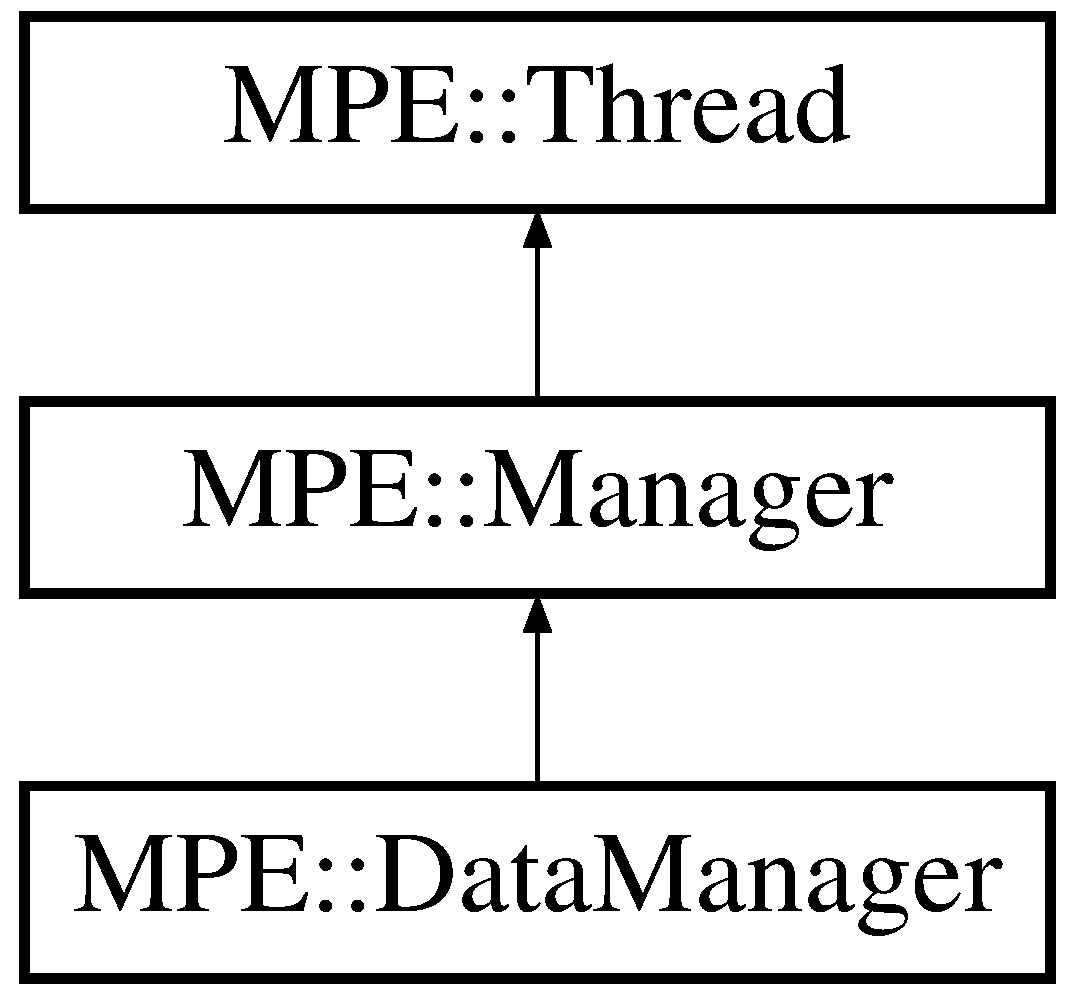
\includegraphics[height=3.000000cm]{class_m_p_e_1_1_thread}
\end{center}
\end{figure}
\subsection*{Public Member Functions}
\begin{DoxyCompactItemize}
\item 
virtual const void \hyperlink{class_m_p_e_1_1_thread_a1bd133a96ec27c868b6bb758e11c0691}{Start} ()=0
\begin{DoxyCompactList}\small\item\em The main entry point for the thread. \end{DoxyCompactList}\item 
\hyperlink{namespace_m_p_e_a16447295e3105bd2ba2a9ea303566175}{thread\+Identifier} \hyperlink{class_m_p_e_1_1_thread_a736d2fc9d527a96419b428e018d225b3}{Get\+Identity} () const
\item 
const void \hyperlink{class_m_p_e_1_1_thread_a1e2ab6a736581d343719f0bba51aa9ad}{Send} (void $\ast$data, uint32\+\_\+t src, uint32\+\_\+t tag, uint8\+\_\+t prio)
\begin{DoxyCompactList}\small\item\em Recvieves message from other thread. \end{DoxyCompactList}\end{DoxyCompactItemize}
\subsection*{Protected Member Functions}
\begin{DoxyCompactItemize}
\item 
\hyperlink{class_m_p_e_1_1_thread_a6b7b08a261115586ae914a9a2325c299}{Thread} (\hyperlink{namespace_m_p_e_a16447295e3105bd2ba2a9ea303566175}{thread\+Identifier} identifier, uint8\+\_\+t frame\+Sync\+Time=16)
\begin{DoxyCompactList}\small\item\em \hyperlink{class_m_p_e_1_1_thread}{Thread} contructor. \end{DoxyCompactList}\item 
virtual \hyperlink{class_m_p_e_1_1_thread_a5addf4f2209106f58447e2c46087c8d7}{$\sim$\+Thread} ()
\item 
const void \hyperlink{class_m_p_e_1_1_thread_a33de6f9fb89f4ae2adf393e866e198da}{Recv} (\hyperlink{struct_m_p_e_1_1_msg}{Msg} \&msg, uint32\+\_\+t src, uint32\+\_\+t tag)
\begin{DoxyCompactList}\small\item\em Recvieve a message. \end{DoxyCompactList}\item 
const uint32\+\_\+t \hyperlink{class_m_p_e_1_1_thread_afa51801ad970ca768ec5160d7c0d7d42}{Peek\+Msg} (\hyperlink{struct_m_p_e_1_1_msg}{Msg} \&msg, uint32\+\_\+t src, uint32\+\_\+t tag)
\begin{DoxyCompactList}\small\item\em Peek message queue. \end{DoxyCompactList}\end{DoxyCompactItemize}
\subsection*{Protected Attributes}
\begin{DoxyCompactItemize}
\item 
\hyperlink{namespace_m_p_e_a16447295e3105bd2ba2a9ea303566175}{thread\+Identifier} \hyperlink{class_m_p_e_1_1_thread_ab7e98443f40fcf9182ea7bf954b8aaf2}{\+\_\+identity}
\item 
uint8\+\_\+t \hyperlink{class_m_p_e_1_1_thread_ad004c47c4002461c874eae460e18ed2a}{\+\_\+frame\+Sync\+Time}
\item 
std\+::priority\+\_\+queue$<$ \hyperlink{struct_m_p_e_1_1_msg}{Msg}, std\+::vector$<$ \hyperlink{struct_m_p_e_1_1_msg}{Msg} $>$, \hyperlink{struct_m_p_e_1_1_msg_comp}{Msg\+Comp} $>$ \hyperlink{class_m_p_e_1_1_thread_a1484f887be46d595bd49c84eef9911ee}{\+\_\+message\+Queue}
\end{DoxyCompactItemize}
\subsection*{Private Attributes}
\begin{DoxyCompactItemize}
\item 
std\+::mutex \hyperlink{class_m_p_e_1_1_thread_af03852c385981359d28bf776370aae3a}{\+\_\+write\+Lock}
\end{DoxyCompactItemize}


\subsection{Detailed Description}
The thread base class. 

This is a virtual class and is intended to be inherited by classes that wishes to use the \hyperlink{class_m_p_e_1_1_thread_message_controller}{Thread\+Message\+Controller}. \begin{DoxySeeAlso}{See also}
\hyperlink{class_m_p_e_1_1_thread_message_controller}{Thread\+Message\+Controller} 
\end{DoxySeeAlso}


\subsection{Constructor \& Destructor Documentation}
\mbox{\Hypertarget{class_m_p_e_1_1_thread_a6b7b08a261115586ae914a9a2325c299}\label{class_m_p_e_1_1_thread_a6b7b08a261115586ae914a9a2325c299}} 
\index{M\+P\+E\+::\+Thread@{M\+P\+E\+::\+Thread}!Thread@{Thread}}
\index{Thread@{Thread}!M\+P\+E\+::\+Thread@{M\+P\+E\+::\+Thread}}
\subsubsection{\texorpdfstring{Thread()}{Thread()}}
{\footnotesize\ttfamily M\+P\+E\+::\+Thread\+::\+Thread (\begin{DoxyParamCaption}\item[{\hyperlink{namespace_m_p_e_a16447295e3105bd2ba2a9ea303566175}{thread\+Identifier}}]{identifier,  }\item[{uint8\+\_\+t}]{frame\+Sync\+Time = {\ttfamily 16} }\end{DoxyParamCaption})\hspace{0.3cm}{\ttfamily [protected]}}



\hyperlink{class_m_p_e_1_1_thread}{Thread} contructor. 


\begin{DoxyParams}{Parameters}
{\em frame\+Sync\+Time} & Limit the thread\textquotesingle{}s frametime to a specific time in ms. \\
\hline
\end{DoxyParams}
\mbox{\Hypertarget{class_m_p_e_1_1_thread_a5addf4f2209106f58447e2c46087c8d7}\label{class_m_p_e_1_1_thread_a5addf4f2209106f58447e2c46087c8d7}} 
\index{M\+P\+E\+::\+Thread@{M\+P\+E\+::\+Thread}!````~Thread@{$\sim$\+Thread}}
\index{````~Thread@{$\sim$\+Thread}!M\+P\+E\+::\+Thread@{M\+P\+E\+::\+Thread}}
\subsubsection{\texorpdfstring{$\sim$\+Thread()}{~Thread()}}
{\footnotesize\ttfamily M\+P\+E\+::\+Thread\+::$\sim$\+Thread (\begin{DoxyParamCaption}{ }\end{DoxyParamCaption})\hspace{0.3cm}{\ttfamily [protected]}, {\ttfamily [virtual]}}



\subsection{Member Function Documentation}
\mbox{\Hypertarget{class_m_p_e_1_1_thread_a736d2fc9d527a96419b428e018d225b3}\label{class_m_p_e_1_1_thread_a736d2fc9d527a96419b428e018d225b3}} 
\index{M\+P\+E\+::\+Thread@{M\+P\+E\+::\+Thread}!Get\+Identity@{Get\+Identity}}
\index{Get\+Identity@{Get\+Identity}!M\+P\+E\+::\+Thread@{M\+P\+E\+::\+Thread}}
\subsubsection{\texorpdfstring{Get\+Identity()}{GetIdentity()}}
{\footnotesize\ttfamily \hyperlink{namespace_m_p_e_a16447295e3105bd2ba2a9ea303566175}{thread\+Identifier} M\+P\+E\+::\+Thread\+::\+Get\+Identity (\begin{DoxyParamCaption}{ }\end{DoxyParamCaption}) const\hspace{0.3cm}{\ttfamily [inline]}}

\mbox{\Hypertarget{class_m_p_e_1_1_thread_afa51801ad970ca768ec5160d7c0d7d42}\label{class_m_p_e_1_1_thread_afa51801ad970ca768ec5160d7c0d7d42}} 
\index{M\+P\+E\+::\+Thread@{M\+P\+E\+::\+Thread}!Peek\+Msg@{Peek\+Msg}}
\index{Peek\+Msg@{Peek\+Msg}!M\+P\+E\+::\+Thread@{M\+P\+E\+::\+Thread}}
\subsubsection{\texorpdfstring{Peek\+Msg()}{PeekMsg()}}
{\footnotesize\ttfamily const uint32\+\_\+t M\+P\+E\+::\+Thread\+::\+Peek\+Msg (\begin{DoxyParamCaption}\item[{\hyperlink{struct_m_p_e_1_1_msg}{Msg} \&}]{msg,  }\item[{uint32\+\_\+t}]{src,  }\item[{uint32\+\_\+t}]{tag }\end{DoxyParamCaption})\hspace{0.3cm}{\ttfamily [protected]}}



Peek message queue. 

This is a non-\/blocking command \begin{DoxySeeAlso}{See also}
\hyperlink{struct_m_p_e_1_1_msg}{Msg} 
\end{DoxySeeAlso}

\begin{DoxyParams}{Parameters}
{\em Src} & Intended destination. Specify \hyperlink{namespace_m_p_e_a0a698f47d1ab10c44a414685c36494f1}{M\+P\+E\+::\+Msg\+\_\+\+Any\+\_\+\+Src} to accept message from any source \\
\hline
{\em tag} & An identifier for the recviever, tags are found in \hyperlink{namespace_m_p_e_1_1_tag}{M\+P\+E\+::\+Tag}, or any user defined tags \\
\hline
\end{DoxyParams}
\begin{DoxyReturn}{Returns}
Returns 0 if no messages in queue, non-\/zero otherwise. 
\end{DoxyReturn}
\begin{DoxySeeAlso}{See also}
\hyperlink{namespace_m_p_e_1_1_tag}{Tag} 
\end{DoxySeeAlso}
\mbox{\Hypertarget{class_m_p_e_1_1_thread_a33de6f9fb89f4ae2adf393e866e198da}\label{class_m_p_e_1_1_thread_a33de6f9fb89f4ae2adf393e866e198da}} 
\index{M\+P\+E\+::\+Thread@{M\+P\+E\+::\+Thread}!Recv@{Recv}}
\index{Recv@{Recv}!M\+P\+E\+::\+Thread@{M\+P\+E\+::\+Thread}}
\subsubsection{\texorpdfstring{Recv()}{Recv()}}
{\footnotesize\ttfamily const void M\+P\+E\+::\+Thread\+::\+Recv (\begin{DoxyParamCaption}\item[{\hyperlink{struct_m_p_e_1_1_msg}{Msg} \&}]{msg,  }\item[{uint32\+\_\+t}]{src,  }\item[{uint32\+\_\+t}]{tag }\end{DoxyParamCaption})\hspace{0.3cm}{\ttfamily [protected]}}



Recvieve a message. 

This is a blocking command. Waits for a specific message. \begin{DoxySeeAlso}{See also}
\hyperlink{struct_m_p_e_1_1_msg}{Msg} 
\end{DoxySeeAlso}

\begin{DoxyParams}{Parameters}
{\em Src} & Intended src. Specify \hyperlink{namespace_m_p_e_a0a698f47d1ab10c44a414685c36494f1}{M\+P\+E\+::\+Msg\+\_\+\+Any\+\_\+\+Src} to accept message from any source \\
\hline
{\em tag} & An identifier for the recviever. \\
\hline
\end{DoxyParams}
\begin{DoxySeeAlso}{See also}
\hyperlink{namespace_m_p_e_1_1_tag}{Tag} 
\end{DoxySeeAlso}
\mbox{\Hypertarget{class_m_p_e_1_1_thread_a1e2ab6a736581d343719f0bba51aa9ad}\label{class_m_p_e_1_1_thread_a1e2ab6a736581d343719f0bba51aa9ad}} 
\index{M\+P\+E\+::\+Thread@{M\+P\+E\+::\+Thread}!Send@{Send}}
\index{Send@{Send}!M\+P\+E\+::\+Thread@{M\+P\+E\+::\+Thread}}
\subsubsection{\texorpdfstring{Send()}{Send()}}
{\footnotesize\ttfamily const void M\+P\+E\+::\+Thread\+::\+Send (\begin{DoxyParamCaption}\item[{void $\ast$}]{data,  }\item[{uint32\+\_\+t}]{src,  }\item[{uint32\+\_\+t}]{tag,  }\item[{uint8\+\_\+t}]{prio }\end{DoxyParamCaption})}



Recvieves message from other thread. 

This is a non-\/blocking command, will continue without wait for message to be delivered. This is called by other threads, not itself. For sending messages see \hyperlink{class_m_p_e_1_1_thread_message_controller_afcc8f572cd1355df9e6a0ef8e2d0f710}{Thread\+Message\+Controller\+::\+Send}. 
\begin{DoxyParams}{Parameters}
{\em data} & Data to be sent \\
\hline
{\em src} & Source \\
\hline
{\em tag} & An identifier for the recviever. \\
\hline
{\em prio} & Priority of the message, 0 is lowest. \\
\hline
\end{DoxyParams}
\begin{DoxySeeAlso}{See also}
\hyperlink{namespace_m_p_e_1_1_tag}{Tag} 
\end{DoxySeeAlso}
\mbox{\Hypertarget{class_m_p_e_1_1_thread_a1bd133a96ec27c868b6bb758e11c0691}\label{class_m_p_e_1_1_thread_a1bd133a96ec27c868b6bb758e11c0691}} 
\index{M\+P\+E\+::\+Thread@{M\+P\+E\+::\+Thread}!Start@{Start}}
\index{Start@{Start}!M\+P\+E\+::\+Thread@{M\+P\+E\+::\+Thread}}
\subsubsection{\texorpdfstring{Start()}{Start()}}
{\footnotesize\ttfamily virtual const void M\+P\+E\+::\+Thread\+::\+Start (\begin{DoxyParamCaption}{ }\end{DoxyParamCaption})\hspace{0.3cm}{\ttfamily [pure virtual]}}



The main entry point for the thread. 



Implemented in \hyperlink{class_m_p_e_1_1_data_manager_aa8d6f1ef687afb532d968a3c1a42f324}{M\+P\+E\+::\+Data\+Manager}.



\subsection{Member Data Documentation}
\mbox{\Hypertarget{class_m_p_e_1_1_thread_ad004c47c4002461c874eae460e18ed2a}\label{class_m_p_e_1_1_thread_ad004c47c4002461c874eae460e18ed2a}} 
\index{M\+P\+E\+::\+Thread@{M\+P\+E\+::\+Thread}!\+\_\+frame\+Sync\+Time@{\+\_\+frame\+Sync\+Time}}
\index{\+\_\+frame\+Sync\+Time@{\+\_\+frame\+Sync\+Time}!M\+P\+E\+::\+Thread@{M\+P\+E\+::\+Thread}}
\subsubsection{\texorpdfstring{\+\_\+frame\+Sync\+Time}{\_frameSyncTime}}
{\footnotesize\ttfamily uint8\+\_\+t M\+P\+E\+::\+Thread\+::\+\_\+frame\+Sync\+Time\hspace{0.3cm}{\ttfamily [protected]}}

\mbox{\Hypertarget{class_m_p_e_1_1_thread_ab7e98443f40fcf9182ea7bf954b8aaf2}\label{class_m_p_e_1_1_thread_ab7e98443f40fcf9182ea7bf954b8aaf2}} 
\index{M\+P\+E\+::\+Thread@{M\+P\+E\+::\+Thread}!\+\_\+identity@{\+\_\+identity}}
\index{\+\_\+identity@{\+\_\+identity}!M\+P\+E\+::\+Thread@{M\+P\+E\+::\+Thread}}
\subsubsection{\texorpdfstring{\+\_\+identity}{\_identity}}
{\footnotesize\ttfamily \hyperlink{namespace_m_p_e_a16447295e3105bd2ba2a9ea303566175}{thread\+Identifier} M\+P\+E\+::\+Thread\+::\+\_\+identity\hspace{0.3cm}{\ttfamily [protected]}}

\mbox{\Hypertarget{class_m_p_e_1_1_thread_a1484f887be46d595bd49c84eef9911ee}\label{class_m_p_e_1_1_thread_a1484f887be46d595bd49c84eef9911ee}} 
\index{M\+P\+E\+::\+Thread@{M\+P\+E\+::\+Thread}!\+\_\+message\+Queue@{\+\_\+message\+Queue}}
\index{\+\_\+message\+Queue@{\+\_\+message\+Queue}!M\+P\+E\+::\+Thread@{M\+P\+E\+::\+Thread}}
\subsubsection{\texorpdfstring{\+\_\+message\+Queue}{\_messageQueue}}
{\footnotesize\ttfamily std\+::priority\+\_\+queue$<$\hyperlink{struct_m_p_e_1_1_msg}{Msg}, std\+::vector$<$\hyperlink{struct_m_p_e_1_1_msg}{Msg}$>$, \hyperlink{struct_m_p_e_1_1_msg_comp}{Msg\+Comp}$>$ M\+P\+E\+::\+Thread\+::\+\_\+message\+Queue\hspace{0.3cm}{\ttfamily [protected]}}

\mbox{\Hypertarget{class_m_p_e_1_1_thread_af03852c385981359d28bf776370aae3a}\label{class_m_p_e_1_1_thread_af03852c385981359d28bf776370aae3a}} 
\index{M\+P\+E\+::\+Thread@{M\+P\+E\+::\+Thread}!\+\_\+write\+Lock@{\+\_\+write\+Lock}}
\index{\+\_\+write\+Lock@{\+\_\+write\+Lock}!M\+P\+E\+::\+Thread@{M\+P\+E\+::\+Thread}}
\subsubsection{\texorpdfstring{\+\_\+write\+Lock}{\_writeLock}}
{\footnotesize\ttfamily std\+::mutex M\+P\+E\+::\+Thread\+::\+\_\+write\+Lock\hspace{0.3cm}{\ttfamily [private]}}



The documentation for this class was generated from the following files\+:\begin{DoxyCompactItemize}
\item 
\hyperlink{_thread_8h}{Thread.\+h}\item 
\hyperlink{_thread_8cpp}{Thread.\+cpp}\end{DoxyCompactItemize}

\hypertarget{class_m_p_e_1_1_thread_message_controller}{}\section{M\+PE\+:\+:Thread\+Message\+Controller Class Reference}
\label{class_m_p_e_1_1_thread_message_controller}\index{M\+P\+E\+::\+Thread\+Message\+Controller@{M\+P\+E\+::\+Thread\+Message\+Controller}}


The \hyperlink{class_m_p_e_1_1_thread_message_controller}{Thread\+Message\+Controller} initiates threads and handles the communication between them.  




{\ttfamily \#include $<$Thread\+Message\+Controller.\+h$>$}

\subsection*{Public Member Functions}
\begin{DoxyCompactItemize}
\item 
const void \hyperlink{class_m_p_e_1_1_thread_message_controller_a08663e963b8ac560e0678527a6f0cd86}{Start\+Thread} (\hyperlink{class_m_p_e_1_1_thread}{Thread} $\ast$thread, double frame\+Sync\+Time)
\begin{DoxyCompactList}\small\item\em Starts a new thread. \end{DoxyCompactList}\item 
const void \hyperlink{class_m_p_e_1_1_thread_message_controller_ad4fdb8a09a50306d1002fd3fb5bae5e3}{Send} (void $\ast$data, size\+\_\+t size, uint32\+\_\+t dest, uint32\+\_\+t tag)
\begin{DoxyCompactList}\small\item\em Send a message. \end{DoxyCompactList}\item 
const void \hyperlink{class_m_p_e_1_1_thread_message_controller_a76ce2d05dfedd82e6d522151d42880f6}{BroadC} (void $\ast$data, size\+\_\+t, uint32\+\_\+t tag)
\begin{DoxyCompactList}\small\item\em Send a Broadcast to all threads. \end{DoxyCompactList}\item 
const void \hyperlink{class_m_p_e_1_1_thread_message_controller_ab55fff1fb40f1456efb7e029fa1ddb89}{Recv} (void $\ast$$\ast$data, size\+\_\+t \&size, uint32\+\_\+t src, uint32\+\_\+t tag)
\begin{DoxyCompactList}\small\item\em Recvieve a message. \end{DoxyCompactList}\item 
const uint32\+\_\+t \hyperlink{class_m_p_e_1_1_thread_message_controller_abfa4aaad59117d2b4f83cf7504d55cb7}{Peek\+Msg} (void $\ast$$\ast$data, size\+\_\+t \&size, uint32\+\_\+t src, uint32\+\_\+t tag)
\begin{DoxyCompactList}\small\item\em Peek message queue. \end{DoxyCompactList}\end{DoxyCompactItemize}


\subsection{Detailed Description}
The \hyperlink{class_m_p_e_1_1_thread_message_controller}{Thread\+Message\+Controller} initiates threads and handles the communication between them. 

\subsection{Member Function Documentation}
\mbox{\Hypertarget{class_m_p_e_1_1_thread_message_controller_a76ce2d05dfedd82e6d522151d42880f6}\label{class_m_p_e_1_1_thread_message_controller_a76ce2d05dfedd82e6d522151d42880f6}} 
\index{M\+P\+E\+::\+Thread\+Message\+Controller@{M\+P\+E\+::\+Thread\+Message\+Controller}!BroadC@{BroadC}}
\index{BroadC@{BroadC}!M\+P\+E\+::\+Thread\+Message\+Controller@{M\+P\+E\+::\+Thread\+Message\+Controller}}
\subsubsection{\texorpdfstring{Broad\+C()}{BroadC()}}
{\footnotesize\ttfamily const void M\+P\+E\+::\+Thread\+Message\+Controller\+::\+BroadC (\begin{DoxyParamCaption}\item[{void $\ast$}]{data,  }\item[{size\+\_\+t}]{,  }\item[{uint32\+\_\+t}]{tag }\end{DoxyParamCaption})}



Send a Broadcast to all threads. 

This is a non-\/blocking command 
\begin{DoxyParams}{Parameters}
{\em data} & Data to be sent \\
\hline
{\em size} & size of data \\
\hline
{\em tag} & An identifier for the recviever. \\
\hline
\end{DoxyParams}
\begin{DoxySeeAlso}{See also}
\hyperlink{struct_tag}{Tag} 
\end{DoxySeeAlso}
\mbox{\Hypertarget{class_m_p_e_1_1_thread_message_controller_abfa4aaad59117d2b4f83cf7504d55cb7}\label{class_m_p_e_1_1_thread_message_controller_abfa4aaad59117d2b4f83cf7504d55cb7}} 
\index{M\+P\+E\+::\+Thread\+Message\+Controller@{M\+P\+E\+::\+Thread\+Message\+Controller}!Peek\+Msg@{Peek\+Msg}}
\index{Peek\+Msg@{Peek\+Msg}!M\+P\+E\+::\+Thread\+Message\+Controller@{M\+P\+E\+::\+Thread\+Message\+Controller}}
\subsubsection{\texorpdfstring{Peek\+Msg()}{PeekMsg()}}
{\footnotesize\ttfamily const uint32\+\_\+t M\+P\+E\+::\+Thread\+Message\+Controller\+::\+Peek\+Msg (\begin{DoxyParamCaption}\item[{void $\ast$$\ast$}]{data,  }\item[{size\+\_\+t \&}]{size,  }\item[{uint32\+\_\+t}]{src,  }\item[{uint32\+\_\+t}]{tag }\end{DoxyParamCaption})}



Peek message queue. 

This is a non-\/blocking command 
\begin{DoxyParams}{Parameters}
{\em data} & Data will be initialized and filled with recvieved data \\
\hline
{\em size} & size of data \\
\hline
{\em Src} & Intended destination. Specify M\+P\+E\+::\+Any\+Src to accept message from any source \\
\hline
{\em tag} & An identifier for the recviever, tags are found in M\+P\+E\+::\+Tag, or any user defined tags \\
\hline
\end{DoxyParams}
\begin{DoxyReturn}{Returns}
Returns 0 if no messages in queue, non-\/zero otherwise. 
\end{DoxyReturn}
\begin{DoxySeeAlso}{See also}
\hyperlink{struct_tag}{Tag} 
\end{DoxySeeAlso}
\mbox{\Hypertarget{class_m_p_e_1_1_thread_message_controller_ab55fff1fb40f1456efb7e029fa1ddb89}\label{class_m_p_e_1_1_thread_message_controller_ab55fff1fb40f1456efb7e029fa1ddb89}} 
\index{M\+P\+E\+::\+Thread\+Message\+Controller@{M\+P\+E\+::\+Thread\+Message\+Controller}!Recv@{Recv}}
\index{Recv@{Recv}!M\+P\+E\+::\+Thread\+Message\+Controller@{M\+P\+E\+::\+Thread\+Message\+Controller}}
\subsubsection{\texorpdfstring{Recv()}{Recv()}}
{\footnotesize\ttfamily const void M\+P\+E\+::\+Thread\+Message\+Controller\+::\+Recv (\begin{DoxyParamCaption}\item[{void $\ast$$\ast$}]{data,  }\item[{size\+\_\+t \&}]{size,  }\item[{uint32\+\_\+t}]{src,  }\item[{uint32\+\_\+t}]{tag }\end{DoxyParamCaption})}



Recvieve a message. 

This is a blocking command 
\begin{DoxyParams}{Parameters}
{\em data} & Data will be initialized and filled with recvieved data \\
\hline
{\em size} & size of data \\
\hline
{\em Src} & Intended destination. Specify M\+P\+E\+::\+Any\+Src to accept message from any source \\
\hline
{\em tag} & An identifier for the recviever. \\
\hline
\end{DoxyParams}
\begin{DoxySeeAlso}{See also}
\hyperlink{struct_tag}{Tag} 
\end{DoxySeeAlso}
\mbox{\Hypertarget{class_m_p_e_1_1_thread_message_controller_ad4fdb8a09a50306d1002fd3fb5bae5e3}\label{class_m_p_e_1_1_thread_message_controller_ad4fdb8a09a50306d1002fd3fb5bae5e3}} 
\index{M\+P\+E\+::\+Thread\+Message\+Controller@{M\+P\+E\+::\+Thread\+Message\+Controller}!Send@{Send}}
\index{Send@{Send}!M\+P\+E\+::\+Thread\+Message\+Controller@{M\+P\+E\+::\+Thread\+Message\+Controller}}
\subsubsection{\texorpdfstring{Send()}{Send()}}
{\footnotesize\ttfamily const void M\+P\+E\+::\+Thread\+Message\+Controller\+::\+Send (\begin{DoxyParamCaption}\item[{void $\ast$}]{data,  }\item[{size\+\_\+t}]{size,  }\item[{uint32\+\_\+t}]{dest,  }\item[{uint32\+\_\+t}]{tag }\end{DoxyParamCaption})}



Send a message. 

This is a non-\/blocking command 
\begin{DoxyParams}{Parameters}
{\em data} & Data to be sent \\
\hline
{\em size} & size of data \\
\hline
{\em dest} & Intended destination \\
\hline
{\em tag} & An identifier for the recviever. \\
\hline
\end{DoxyParams}
\begin{DoxySeeAlso}{See also}
\hyperlink{struct_tag}{Tag} 
\end{DoxySeeAlso}
\mbox{\Hypertarget{class_m_p_e_1_1_thread_message_controller_a08663e963b8ac560e0678527a6f0cd86}\label{class_m_p_e_1_1_thread_message_controller_a08663e963b8ac560e0678527a6f0cd86}} 
\index{M\+P\+E\+::\+Thread\+Message\+Controller@{M\+P\+E\+::\+Thread\+Message\+Controller}!Start\+Thread@{Start\+Thread}}
\index{Start\+Thread@{Start\+Thread}!M\+P\+E\+::\+Thread\+Message\+Controller@{M\+P\+E\+::\+Thread\+Message\+Controller}}
\subsubsection{\texorpdfstring{Start\+Thread()}{StartThread()}}
{\footnotesize\ttfamily const void M\+P\+E\+::\+Thread\+Message\+Controller\+::\+Start\+Thread (\begin{DoxyParamCaption}\item[{\hyperlink{class_m_p_e_1_1_thread}{Thread} $\ast$}]{thread,  }\item[{double}]{frame\+Sync\+Time }\end{DoxyParamCaption})}



Starts a new thread. 


\begin{DoxyParams}{Parameters}
{\em thread} & Pointer to the class which should occupy the thread \\
\hline
{\em frame\+Sync\+Time} & Limit the thread\textquotesingle{}s frametime to a specific time. \\
\hline
\end{DoxyParams}
\begin{DoxySeeAlso}{See also}
\hyperlink{class_m_p_e_1_1_thread}{Thread} 
\end{DoxySeeAlso}


The documentation for this class was generated from the following files\+:\begin{DoxyCompactItemize}
\item 
Thread\+Message\+Controller.\+h\item 
Thread\+Message\+Controller.\+cpp\end{DoxyCompactItemize}

%--- End generated contents ---

% Index
\backmatter
\newpage
\phantomsection
\clearemptydoublepage
\addcontentsline{toc}{chapter}{Index}
\printindex

\end{document}
